\section{通用场景的图像视频修复}
\label{sec:other}

\subsection{光流引导的端到端视频修复}

针对水印去除的图像视频修复工作相对较少,更多的是通用的图像视频修复任务,过去的工作也多有采用图像视频修复方法作为水印去除的主要技术手段或细化方法。之前的视频补全方法,大致可以分为三类:第一类为非深度学习时代的Patch-borrowing的方法,这类方法先根据输入视频或外部数据建立一个volume,每个待补全的图像块都会在这个volume中寻找相似的图像块来更新待补全的区域。第二类为深度学习时代中基于autoencoder的方法,这类方法主要依托于类U-Net的网络结构,这其中会引入比如说3d convolution、gated convolution或是在bottleneck的地方使用transformer来进行端到端的视频补全。第三类为基于光流的方法。

基于光流的方法将视频补全看作是像素传播的过程,其主要包含了三个阶段,第一阶段为光流补全,由于mask掉的区域光流是无法直接估计的,所以就需要借助mask外区域的光流来对缺失的部分进行补全。光流由于其结构和纹理都相比视频简单,所以光流补全要比视频补全容易得多。第二阶段为像素传播,借助补全后的双向光流来索引邻近帧中对应的像素对缺失部分补全。第三步为内容幻化,对于传播过程中没有索引到的区域,通过一个预训练的图像补全网络来完成最后的填充。这三个阶段是分别执行的,并不是端到端的,这样一个视频补全系统存在许多缺点:由于第一个阶段与第二个阶段存在许多复杂的手工设计的操作,因此计算效率很低,处理70帧的不到360p的视频就需要约4分钟。同时由于这三个阶段是分别执行的,每个阶段都非常依赖上个阶段的生成的结果,因此容易造成误差的累积与放大。最后一阶段所使用图像补全网络只考虑了单帧信息,因此生成的结果时间及空间的一致性不是很高。

为解决上述问题,Li等~\cite{li2022towards}希望模拟之前基于光流引导的方法的三个阶段,去设计对应的三个模块,以构建一个可以被端到端优化的视频补全框架。首先,将像素传播过程转换为了通过光流引导的特征传播过程。其次将负责光流补全的网络嵌入整个网络框架中,通过额外的光流补全损失使其与其他网络模块一同被端到端地优化。最后在内容幻化模块中,使用temporal focal transformer同时融合局部邻域与非局部视频帧的信息。

\begin{figure*}[!htbp]
	\centering
	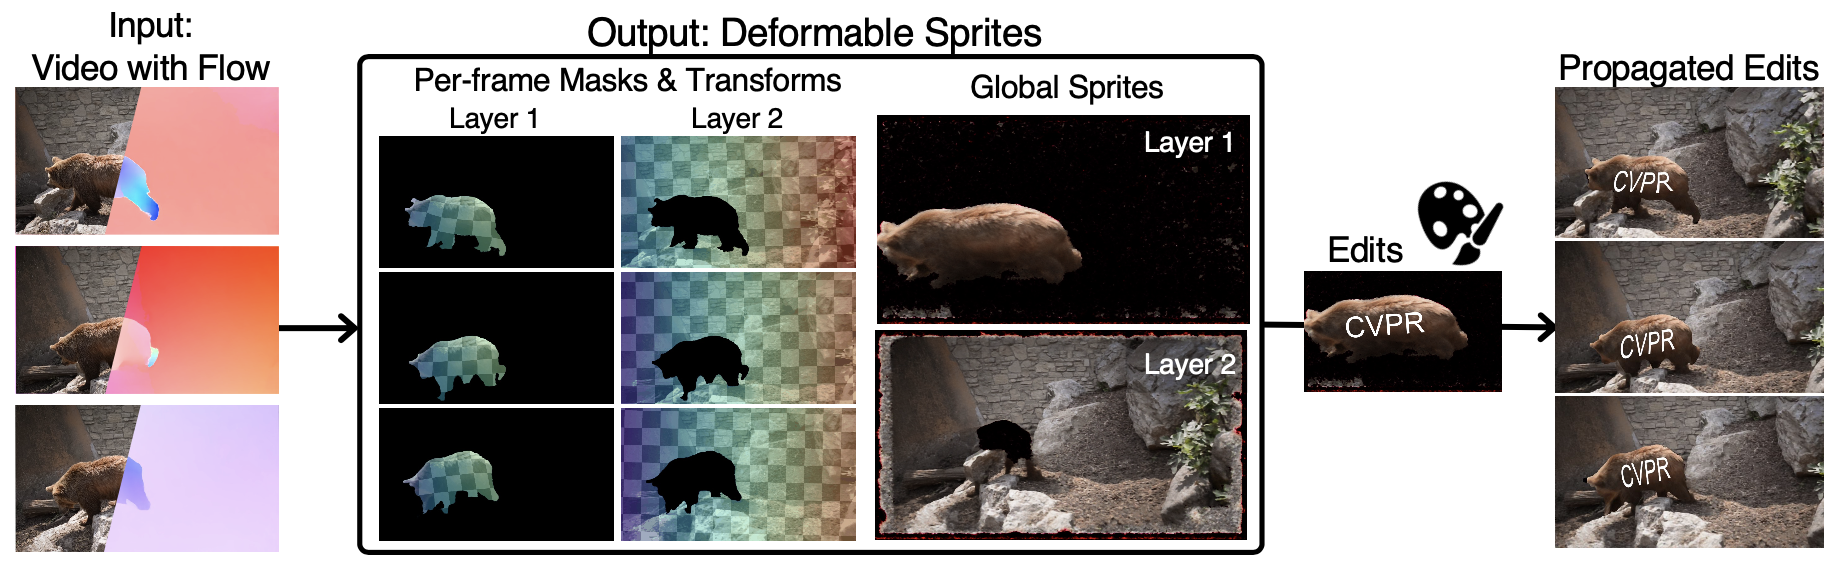
\includegraphics[width=\linewidth]{37.png}
	\caption{光流引导的端到端视频修复网络架构图}
	\label{fig:37}
\end{figure*}

\begin{figure}[!htbp]
	\centering
	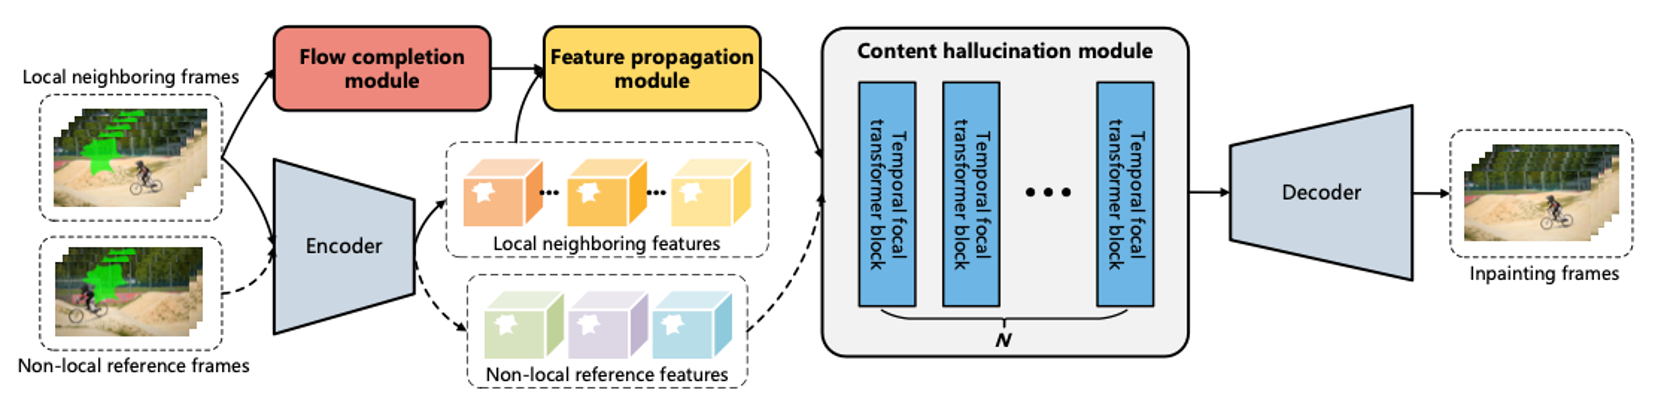
\includegraphics[width=\columnwidth]{35.png}
	\caption{光流引导的端到端视频修复网络架构图}
	\label{fig:35}
\end{figure}

为了实现端到端的光流补全,首先将一个用于光流估计的网络嵌入整个网络框架中作为光流补全模块,并使用额外的光流补全损失来监督。通过这一监督,可以让该光流补全模块同时完成光流的估计与补全。简单起见,我们使用L1 loss来对光流补全模块输出的双向光流进行监督。整个围绕光流补全模块的设计有两点优势:一是该损失可以配合网络其他任务导向的损失一同约束该模块的优化,让这一模块生成任务导向的光流。二是仅需要一个光流估计的子网络就可以直接进行光流的补全,整个光流补全的过程也相较之前的方法更加高效,大约可以快出40倍。

\begin{figure}[!htbp]
	\centering
	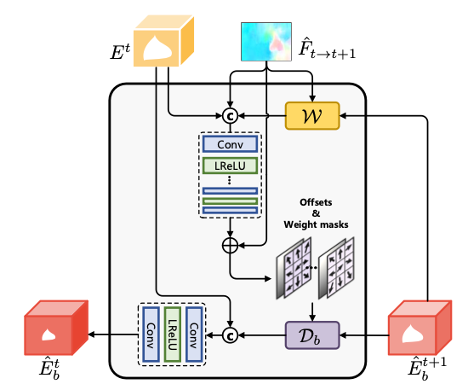
\includegraphics[width=0.9\columnwidth]{36.png}
	\caption{光流引导的可变性卷积结构图}
	\label{fig:35}
\end{figure}

得到补全的光流后,可以将邻近帧的特征根据光流进行索引并warp,进而实现特征的传播。但由于补全后的光流肯定没办法做到100\%准确,不准确的光流信息会导致在特征传播过程中引入无关的信息,进而影响最终的结果。为此,引入deformable convolution来补救这些不好的光流补全结果。Deformable convolution可以让sample点的位置更多更灵活,同时自适应地汇聚这些信息,使特征传播过程更加有效。而光流可以为deformable convolution给出更好的起始sample点选择,使其更容易sample到有意义的内容信息。

在inpainting中为了补全缺失部分的信息,一种很朴素的想法就是全局暴力搜索相似图像块,但这样的方式计算复杂度高,计算效率很低。对于一块缺失区域而言,与其最相似的内容应该在其周围,越远的区域与其内容越不相似。之前也有一些image inpainting的工作,通过设计权重,在进行填充的时候,mask周围的区域权重大,离mask远的区域权重小。本文使用了focal attention,即在局部区域使用细粒度的attention,在全局使用粗粒度的attention。